\documentclass[a4paper]{jsarticle}
\setlength{\topmargin}{-20.4cm}
\setlength{\oddsidemargin}{-10.4mm}
\setlength{\evensidemargin}{-10.4mm}
\setlength{\textwidth}{18cm}
\setlength{\textheight}{26cm}

\usepackage[top=15truemm,bottom=25truemm,left=20truemm,right=20truemm]{geometry}
\usepackage[latin1]{inputenc}
\usepackage{amsmath}
\usepackage{amsfonts}
\usepackage{amssymb}
\usepackage[dvipdfmx]{graphicx}
\usepackage[dvipdfmx]{color}
\usepackage{listings}
\usepackage{listings,jvlisting}
\usepackage{geometry}
\usepackage{framed}
\usepackage{color}
\usepackage[dvipdfmx]{hyperref}
\usepackage{ascmac}
\usepackage{enumerate}
\usepackage{tabularx}
\usepackage{cancel}
\usepackage{scalefnt}

\renewcommand{\figurename}{fig.}
\renewcommand{\tablename}{table }
\newcommand{\redunderline}[1]{\textcolor{BrickRed}{\underline{\textcolor{black}{#1}}}} 

\hypersetup{
	colorlinks=false, % リンクに色をつけない設定
	bookmarks=true, % 以下ブックマークに関する設定
	bookmarksnumbered=true,
	pdfborder={0 0 0},
	bookmarkstype=toc
}

\lstset{
basicstyle={\ttfamily},
identifierstyle={\small},
commentstyle={\smallitshape},
keywordstyle={\small\bfseries},
ndkeywordstyle={\small},
stringstyle={\small\ttfamily},
frame={tb},
breaklines=true,
columns=[l]{fullflexible},
xrightmargin=0zw,
xleftmargin=3zw,
numberstyle={\scriptsize},
stepnumber=1,
numbersep=1zw,
lineskip=-0.5ex
}

\setcounter{tocdepth}{3}

\author{}
\title{材料力学}
\date{}

\begin{document}
\maketitle
\tableofcontents
\newpage

\section{引張・圧縮}
\begin{itembox}[l]{重要公式}
    \begin{center}
        \begin{eqnarray*}
            \sigma&=&\dfrac{P}{A}\\
            \varepsilon&=&\dfrac{\lambda}{L}\\
            \sigma&=&E\varepsilon\\
            P&=&\dfrac{AE}{l}\lambda=AE\varepsilon\\
            AE&:&引張剛性\\
        \end{eqnarray*}
    \end{center}
\end{itembox}
\subsection{微小区間のひずみ}
\begin{itembox}[l]{微小区間のひずみ}
    \begin{eqnarray*}
        d\varepsilon=\dfrac{d\lambda}{dx}\\
    \end{eqnarray*}
\end{itembox}
\subsection{ポアソン比}
例えば丸棒を引張ると引張方向に\textgt{縦ひずみ}が発生し,同時に径が小さくなる\textgt{横ひずみ}が発生する.\\
このときの縦ひずみと横ひずみの比を\textgt{ポアソン比}という.
\begin{itembox}[l]{ポアソン比}
    \begin{center}
        $x$軸方向に材料に力を加えるとき
    \end{center}
    \begin{eqnarray*}
        \nu=-\dfrac{\left(横ひずみ\right)}{\left(縦ひずみ\right)}=-\dfrac{\varepsilon_y}{\varepsilon_x}\\
    \end{eqnarray*}
    \begin{center}
        ※ 「$-$」は,ポアソン比の値を正にするため
    \end{center}
\end{itembox}
\begin{itembox}[l]{ポアソン比と応力・ひずみの関係式}
    \begin{eqnarray*}
        \varepsilon_x&=&\dfrac{\sigma_x}{E}\\
        \varepsilon_y&=&-\nu\dfrac{\sigma_x}{E}\\
    \end{eqnarray*}
\end{itembox}
\begin{itembox}[l]{ポアソン比と弾性係数の関係}
    \begin{eqnarray*}
        E=2G\left(1+\nu\right)\\
    \end{eqnarray*}
\end{itembox}
\section{ねじり・せん断応力}
\begin{itembox}[l]{重要公式}
    \begin{center}
        \begin{eqnarray*}
            \tau\left(r\right)&=&\dfrac{T}{I_p} r\\
            \gamma\left(r\right)&=&\dfrac{\lambda\left(r\right)}{L}=\dfrac{\varphi}{L}r=\theta r\\
            \tau\left(r\right)&=&G\gamma\left(r\right)=G\theta r\\
            T&=&\dfrac{I_pG}{L}\varphi\\
            I_p&:&断面二次極モーメント\\
            \theta=\dfrac{\varphi}{L}&:&比ねじれ角\\
            I_pG&:&ねじれ剛性\\
        \end{eqnarray*}
    \end{center}
\end{itembox}
\subsection{微小区間のねじれ角}
\begin{itembox}[l]{微小区間のねじれ角}
    \begin{eqnarray*}
        d\gamma=\dfrac{rd\varphi}{dx}\\
    \end{eqnarray*}
\end{itembox}
\section{曲げ}
\begin{itembox}[l]{重要公式}
    \begin{center}
        \begin{eqnarray*}
            \sigma_z\left(z\right)&=&\dfrac{M}{I}z\\
            I&:&\;断面二次モーメント\\
        \end{eqnarray*}
    \end{center}
\end{itembox}
\section{平等強さ}
どの断面でも\textgt{応力が一定}である状態のことをいう.\\
\begin{itembox}[l]{平等強さ}
    \begin{enumerate}[(1)]
        \item 引張・圧縮 $\rightarrow$ どの断面でも\textgt{垂直応力}が等しい
        \item 曲げ $\rightarrow$ どの断面でも\textgt{最大曲げ応力}が等しい
    \end{enumerate}
\end{itembox}
\section{断面二次モーメントと断面二次極モーメント}
\begin{itembox}[l]{Point}
    \begin{center}
        断面二次極モーメントは直交座標系における\textgt{$x$軸,$y$軸の断面二次モーメントを足し合わせた値}になる.\\
        ねじりと曲げの重要公式に酷似しているものが多い.
    \end{center}
\end{itembox}
\subsection{断面二次モーメント}
断面二次モーメントは,部材の断面形状の特性を表した値であり,
その形状が曲げに対してどのくらい\textgt{硬い}のかを表す.
\begin{itembox}[l]{断面二次モーメント}
    \begin{eqnarray*}
        \displaystyle I=\int_Az^2dA\\
    \end{eqnarray*}
\end{itembox}
\begin{itembox}[l]{代表的な断面二次モーメント}
    \begin{eqnarray*}
        長方形\quad&&\dfrac{bh^3}{12}\quad(高さ:h,幅:b)\\
        円\qquad&&\dfrac{\pi D^4}{64}\quad(直径:D)\\
        三角形\quad&&\dfrac{bh^3}{36}\quad(高さ:h,幅:b)\\
    \end{eqnarray*}
\end{itembox}
\subsection{断面二次モーメントの求め方}
\begin{itembox}[l]{断面二次モーメントを求める具体的なステップ}
    \begin{enumerate}[(1)]
        \item 計算の基準になる$z$軸を決定する
        \item 微小面積$dA$を求める
        \item 基準の$z$軸に関して$I_z=\int_Az^2dA$を求める
        \item 平行軸の定理を用いて解を求める
    \end{enumerate}
\end{itembox}
\subsection{平行軸の定理}
図心基準の断面二次モーメントから任意の軸基準の断面二次モーメントを求めるときに利用することができる.
\begin{itembox}[l]{平行軸の定理}
    調べる断面形状(断面積:$A$)の中立軸を$z$軸,それに平行に$z$だけ離れた位置の軸を$z'$軸とする.\\
    中立軸に対する断面二次モーメントを$I_z$,$z$だけ離れた位置の断面二次モーメントを$I_{z'}$とすると,
    以下のように表すことができる.
    \begin{eqnarray*}
        I_{z'}=I_z+Az^2\\
    \end{eqnarray*}
\end{itembox}
\subsection{断面二次極モーメント}
半径$r$に関する(極座標に関する)断面二次モーメントのことを\textgt{断面二次極モーメント}という.
\begin{itembox}[l]{断面二次極モーメント}
    \begin{eqnarray*}
        \displaystyle I_p=\int r^2dA
    \end{eqnarray*}
\end{itembox}
ここで,$x=r\cos\theta,y=\sin\theta$とすると,$r^2=x^2+y^2$と表せるので,
\begin{eqnarray*}
    \displaystyle I_p=\int r^2dA=\int \left(x^2+y^2\right)dA=\int x^2dA+\int y^2dA\\
\end{eqnarray*}
ここで,ある図形に対して直交座標系を考え,$x$軸及び$y$軸における断面二次モーメントをそれぞれ$I_x,I_y$とすると,
\begin{eqnarray*}
    \displaystyle
    I_x&=&\int x^2dAa\\
    I_y&=&\int y^2dA\\
\end{eqnarray*}
であるので,断面二次極モーメントは以下のように表すことができる.
\begin{eqnarray*}
    I_p=I_x+I_y
\end{eqnarray*}
したがって,断面二次極モーメントは直交座標系における\textgt{$x$軸,$y$軸の断面二次モーメントを足し合わせた値}になる.\\
\begin{itembox}[l]{代表的な断面二次極モーメント}
    \begin{eqnarray*}
        円\qquad&&\dfrac{\pi D^4}{32}\quad(直径:D)\\
        円筒\quad&&\dfrac{\pi}{32}\left(D_1^2-D_2^2\right)\quad(外径:D_1,内径:D_2)\\
    \end{eqnarray*}
\end{itembox}
\section{たわみの微分方程式}
\begin{itembox}[l]{たわみの微分方程式}
    \begin{eqnarray*}
        \dfrac{d^2w}{dx^2}&=&-\dfrac{M}{EI}\\
        \dfrac{dw}{dx}&=&\theta\left(x\right):たわみ角 (1回積分)\\
        &&w\left(x\right):たわみ(2回積分)\\
    \end{eqnarray*}
\end{itembox}
\begin{itembox}[l]{境界条件}
    \begin{enumerate}[(1)]
        \item 剛体壁\\
              $x=0$のとき,\quad$\omega=0,\;\theta=0$
        \item 支点\\
              $x=0$のとき,\quad$\omega=0$,力の加わっている個所で$\;\theta =0$
    \end{enumerate}
\end{itembox}
\section{線膨張係数と熱応力}
\begin{itembox}[l]{熱ひずみの公式}
    \begin{eqnarray*}
        \varepsilon=\alpha\Delta T\\
    \end{eqnarray*}
\end{itembox}

\subsection{(例題) 熱応力問題を解く}
\begin{figure}[htbp]
    \begin{center}
        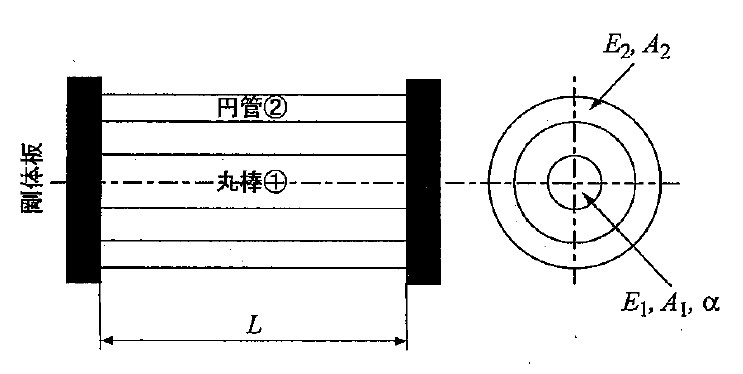
\includegraphics[width=120mm]{images/zairiki_image4.jpg}
        \caption{H24 試験問題 [1]}
    \end{center}
\end{figure}
\begin{enumerate}[(1)]
    \item \textgt{丸棒1に生じるひずみ$\varepsilon_1$を求める}
          \begin{itembox}[l]{Point}
              \begin{center}
                  材料が温度$\Delta T$だけ上昇すると,ひずみに$\alpha \Delta T$が追加される\\
                  (\textgt{合計のひずみ} $\varepsilon'$) = (\textgt{温度上昇によるひずみ} $\alpha \Delta T$) + (\textgt{応力(外力)によるひずみ} $\varepsilon$ )
              \end{center}
          \end{itembox}
          ここで,熱ひずみ$\varepsilon_T$は温度$T$だけ上昇したとき,
          \begin{eqnarray*}
              \varepsilon_T=\alpha T
          \end{eqnarray*}
          また,応力によるひずみ$\varepsilon_\sigma$は
          \begin{eqnarray*}
              \varepsilon_\sigma=\frac{\sigma_1}{E_1}
          \end{eqnarray*}
          したがって,丸棒1のひずみ$\varepsilon_1$は
          \begin{eqnarray*}
              \varepsilon_1&=&\varepsilon_T+\varepsilon_\sigma\\
              &=&\alpha T+\dfrac{\sigma_1}{E_1}
          \end{eqnarray*}
    \item \textgt{丸棒1に生じる応力$\sigma_1$を求める}\\
          \begin{itembox}[l]{Point}
              \begin{center}
                  $\sigma_2$を$\sigma_1$を用いた式で表す
              \end{center}
          \end{itembox}
          力のつり合いより,
          \begin{eqnarray*}
              \sigma_1A_1+\sigma_2A_2=0
          \end{eqnarray*}
          また,伸びは合わせて丸棒1の熱膨張分であるので,
          \begin{eqnarray*}
              \lambda_1+\lambda_2&=&0\\
              \lambda_1&=&-\lambda_2
          \end{eqnarray*}
          両辺を丸棒1,円管2の長さ$L$で割ると,ひずみのつり合いとなる.
          \begin{eqnarray*}
              \frac{\lambda_1}{L}&=&-\frac{\lambda_2}{L}\\
              \varepsilon_1&=&-\varepsilon_2
          \end{eqnarray*}
          したがって,
          \begin{eqnarray*}
              \varepsilon_2&=&-\varepsilon_1=-\left(\alpha T+\dfrac{\sigma_1}{E_1}\right)\\
              \sigma_2&=&E_2\varepsilon_2=-E_2\left(\alpha T+\dfrac{\sigma_1}{E_1}\right)
          \end{eqnarray*}
          これを,力のつり合いの式に代入して整理すると
          \begin{eqnarray*}
              \sigma_1=-\frac{E_1E_2A_2\alpha T}{E_1A_1+E_2A_2}
          \end{eqnarray*}
\end{enumerate}
\section{SFDとBMD (未完成)}
\subsection{せん断力線図(SFD)}
はりにはたらくせん断力を図で表したもの
\begin{itembox}[l]{Point}
    \begin{center}
        該当する範囲で、\textgt{力のつり合い式}を立てる
    \end{center}
\end{itembox}
\subsection{曲げ応力線図(BMD)}
はりにはたらく曲げモーメントを図で表したもの
\begin{itembox}[l]{Point}
    \begin{center}
        該当する範囲で、\textgt{モーメントのつり合い式}を立てる
    \end{center}
\end{itembox}
\begin{enumerate}[(1)]
    \item 自由端の曲げモーメントは\textgt{ゼロ}
    \item 曲げモーメントが最大となる断面を\textgt{危険断面}という
\end{enumerate}
\subsection{(例題) BMDとSFDを書く}

\section{不静定問題}
\begin{itembox}[l]{条件}
    \begin{enumerate}[(1)]
        \item 力・トルクのつり合い
        \item 伸び・ねじれ角のつり合い
    \end{enumerate}
\end{itembox}
\begin{itembox}[l]{Point}
    \begin{center}
        \textgt{力・トルク}のつり合いから\textgt{伸び・ねじれ角}を含む式に変換する
    \end{center}
\end{itembox}
\subsection{(例題) 不静定問題を解く}
\begin{figure}[htbp]
    \begin{center}
        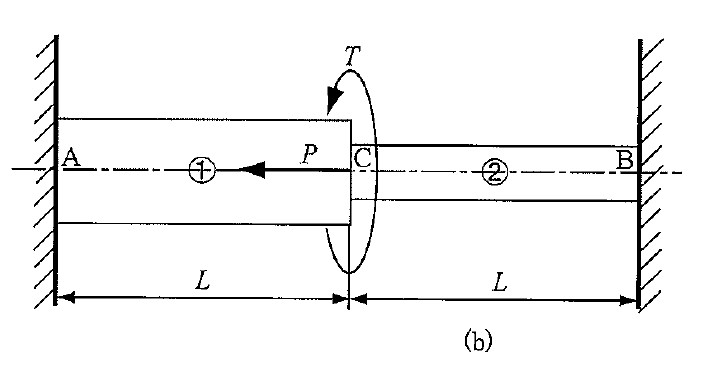
\includegraphics[width=120mm]{images/zairiki_image3.jpg}
        \caption{H27 試験問題 [1]}
    \end{center}
\end{figure}
\begin{enumerate}[(1)]
    \item \textgt{$x=L$に荷重$P$が加わっているときの丸棒2の伸び$\lambda_2$を求める.}\\
          \\
          力のつり合いより,
          \begin{eqnarray*}
              \sigma_1A_1+\sigma_2A_2=P
          \end{eqnarray*}
          伸びは合計でゼロになるので,
          \begin{eqnarray*}
              \lambda_1+\lambda_2&=&0\\
              \lambda_1&=&-\lambda_2
          \end{eqnarray*}
          ここで,応力$\sigma_1,\sigma_2$は,伸び$\lambda_1,\lambda_2$を用いて
          \begin{eqnarray*}
              \sigma_1&=&E\frac{\lambda_1}{L}\\
              \sigma_2&=&E\frac{\lambda_2}{L}
          \end{eqnarray*}
          と表せることから,力のつり合い式に代入すると,
          \begin{eqnarray*}
              E\frac{\lambda_2}{L}A_1+E\frac{\lambda_2}{L}A_2=P
          \end{eqnarray*}
          したがって,
          \begin{eqnarray*}
              \frac{E}{L}\left(\lambda_1A_1+\lambda_2A_2\right)&=&P\\
              \frac{E}{L}\lambda_2\left(A_2-A_1\right)&=&P\\
              \lambda_1&=&\frac{PL}{E\left(A_2-A_1\right)}
          \end{eqnarray*}\\
    \item \textgt{$x=L$にトルク$T$が加わっているときの丸棒2のねじれ角$\varphi_2$を求める.}\\
          \\
          トルクのつり合いより,
          \begin{eqnarray*}
              T_1+T_2=T
          \end{eqnarray*}
          ねじり角は合わせてゼロになるので,
          \begin{eqnarray*}
              \varphi_1+\varphi_2&=&0\\
              \varphi_1&=&-\varphi_2
          \end{eqnarray*}
          ここで,トルク$T_1,T_2$はねじれ角$\varphi_1,\varphi_2$を用いて,
          \begin{eqnarray*}
              T_1&=&I_{P1}G\frac{\varphi_1}{L}\\
              T_2&=&I_{P1}G\frac{\varphi_2}{L}\\
          \end{eqnarray*}
          と表せることから,トルクのつり合い式に代入すると,
          \begin{eqnarray*}
              I_{P1}G\frac{\varphi_1}{L}+I_{P2}G\frac{\varphi_2}{L}=T
          \end{eqnarray*}
          したがって,
          \begin{eqnarray*}
              \frac{G}{L}\left(I_{P1}\varphi_1+I_{P2}\varphi_2\right)&=&T\\
              \frac{G}{L}\varphi_2\left(I_{P2}-I_{P1}\right)&=&T\\
              \varphi_2&=&\frac{TL}{G\left(I_{P2}-I_{P1}\right)}
          \end{eqnarray*}
\end{enumerate}
\section{モールの応力円 (未完成)}
\section{材料の破断}
塑性変形するときは金属材料が単軸応力状態で変形することはなく,2軸または3軸の応力を受けている.
このような組合せ応力のもとにおいて金属材料が弾性限度に達し,
塑性変形を開始するときの条件を降伏条件という.\\
$\sigma_Y$を材料の降伏強度として代表的な降伏条件式を以下に示す.
\subsection{最大主応力説}
この破損則は脆性材料に一致することが多い.
\begin{itembox}[l]{最大主応力説}
    \begin{eqnarray*}
        \sigma_1\geq\sigma_Y\\
    \end{eqnarray*}
\end{itembox}
\subsection{最大せん断応力説}
この破損則は,延性材料に一致することが多い.Trescaの説とも呼ばれる.
\begin{itembox}[l]{最大せん断応力説}
    \begin{eqnarray*}
        \dfrac{\sigma_1-\sigma_3}{2}\geq\dfrac{\sigma_Y}{2}\\
    \end{eqnarray*}
\end{itembox}
\subsection{せん断ひずみエネルギー説}
この破損則は,延性材料に一致することが多い.Von-Misesの説とも呼ばれる.
\begin{itembox}[l]{せん断ひずみエネルギー説}
    \begin{eqnarray*}
        \dfrac{1}{2}\left[\left(\sigma_3-\sigma_1\right)^2+\left(\sigma_1-\sigma_2\right)^2+\left(\sigma_2-\sigma_3\right)^2\right]\geq\left(\sigma_Y\right)^2\\
    \end{eqnarray*}
\end{itembox}
\section{薄肉円筒}
\begin{figure}[htbp]
    \begin{center}
        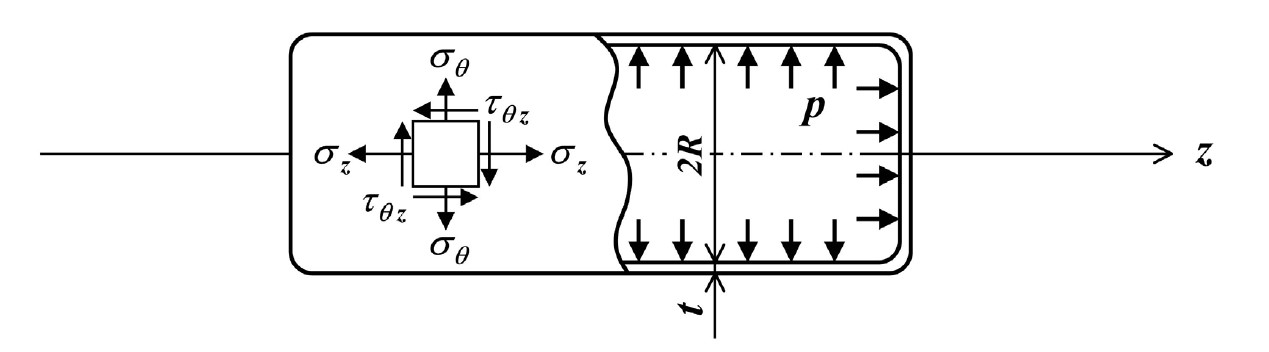
\includegraphics[width=150mm]{images/zairiki_image1.jpg}
        \caption{材料力学2 講義資料1}
    \end{center}
\end{figure}
薄肉とは,上図の内半径$R$に比べて,板厚$t$が十分に小さい,すなわち$t/R \geqq 0.1$のとき程度の場合を指す.\\
このとき,以下の近似が成り立つものとする.
\begin{enumerate}[(1)]
    \item 半径方向応力$\sigma_r$は無視できる
    \item 周方向応力$\sigma_\theta$は板厚に沿って一様である
\end{enumerate}
\subsection{それぞれの応力を求める}
周方向応力$\sigma_r$は近似が成立することから,
\begin{eqnarray*}
    \sigma_r=0
\end{eqnarray*}
\begin{figure}[htbp]
    \begin{center}
        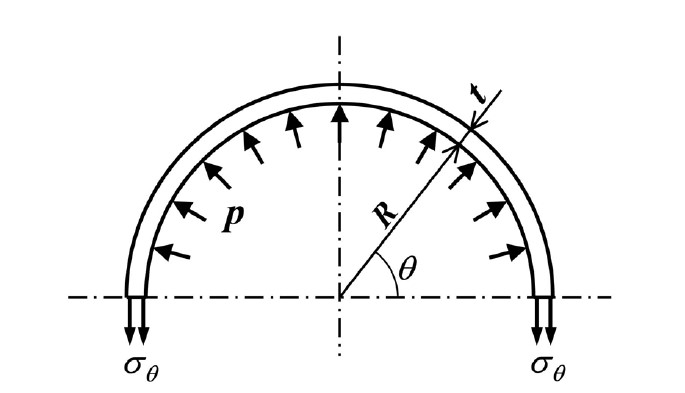
\includegraphics[width=100mm]{images/zairiki_image2.jpg}
        \caption{材料力学2 講義資料2}
    \end{center}
\end{figure}
上図は,円筒を切断したものであり,図の上下方向の力のつり合いより,周方向応力$\sigma_\theta$は,
\begin{eqnarray*}
    \displaystyle
    2t\sigma_\theta &=& \int^\pi_0 pR\sin\theta d\theta = 2pR\\
    \sigma_\theta &=&\dfrac{pr}{t}
\end{eqnarray*}
また,軸方向応力$\sigma_z$は$z$方向の力のつり合いより,
\begin{eqnarray*}
    2\pi Rt \sigma_z&=& \pi R^2p\\
    \sigma_z&=&\dfrac{pr}{2t}
\end{eqnarray*}
したがって,内圧$p$を受ける薄肉円筒に加わる応力は,
\begin{itembox}[l]{薄肉円筒に働く応力}
    \begin{eqnarray*}
        \sigma_r=0\quad
        \sigma_\theta =\dfrac{pr}{t}\quad
        \sigma_z=\dfrac{pr}{2t}
    \end{eqnarray*}
\end{itembox}
なお,外力として荷重$Q$とトルク$T$を受けている場合は,
以上の円筒に生じる応力に,荷重$Q$による垂直応力とトルク$T$によるせん断応力を加えれば良い.

\end{document}